% 爬升的诚实读数。数字全部由 data/ledger/service.db 的 HUMAN 角色事件重算，
% 重算脚本与 scripts/build_figures.py 的 qualifying_climb() 同一判别口径。

\subsection{先说清用哪把尺}
问「这套系统到底有没有在进步」，答案完全取决于计分方式。本报告的计分方式是
\textbf{奖励}：一条构造的 $|t|$ 减去它所在族的零假设地板 $E_2(n)$（\S\ref{sec:selection}）。
奖励为正表示该读数高过「同样多次无关搜索也会达到的高度」，为负表示它连这个高度都没到。
地板随族内分母 $n$ 上升，因此同一条构造在不同时点的奖励不同，报表必须声明用的是哪个地板。

在此之上还有两道过滤，它们决定了哪些成绩\textbf{有资格}被算作证据。
其一是\textbf{数据源}：特征规格里引用了 \path{pm_market}（即 Polymarket 数据）的才算另类数据，
只用期货自身量价算出的构造属基线对照，用于识别假象，不计入另类数据清单。
其二是\textbf{符号一致}：每条假设在读取结果之前冻结了方向（$+1$ 或 $-1$），
实得斜率符号必须与之相同。方向反了而只看绝对值，等于把一条被证否的机制改写成一条事后的相反假设。
表~\ref{tab:threescales} 给出三种口径下各族的最好成绩。

\begin{table}[htbp]\centering\footnotesize
\begin{tabular}{@{}>{\raggedright\arraybackslash}p{0.22\textwidth}
>{\raggedright\arraybackslash}p{0.24\textwidth}
>{\raggedright\arraybackslash}p{0.22\textwidth}
>{\raggedright\arraybackslash}p{0.24\textwidth}@{}}\toprule
口径 & 旧族（地板 2.8622） & 事件条件族（2.3808） & 机制先验族（2.4686） \\ \midrule
全部构造 & 9.30（\path{run5-study-2}），奖励 $+6.44$ &
  1.87（\path{run24-study-2}），$-0.51$ & 3.74（\path{run30-study-5}），$+1.28$ \\
只计另类数据 & 4.89（\path{run6-study-6}），$+2.03$ &
  1.87（同上），$-0.51$ & 3.74（同上），$+1.28$ \\
另类数据且符号一致 & 4.39（\path{run16-study-3}），$+1.53$ &
  1.73（\path{run23-study-7}），$-0.65$ & 1.47（\path{run29-study-6}），$-1.00$ \\
\bottomrule\end{tabular}
\caption{三种口径下各族的最好成绩。奖励取 $|t|$ 减\textbf{本族当前地板}，
地板由 \texttt{expected\_max\_abs\_z} 按当前分母实算：旧族 135、事件条件族 33、
机制先验族 42（机制族另按决定 0013 第四节预注册的全批证否线 $E_2(82)=2.7000$ 结算，
该决定把本批回合定为 40、预算末分母上界定为 $42+40=82$）。
口径每严一档，最好成绩就掉一截：旧族由 9.30 降到 4.39，机制族由 3.74 降到 1.47。}
\label{tab:threescales}
\end{table}

\subsection{三个高分逐条查下来都不成立}
表~\ref{tab:threescales} 第一、二行的三个高分，账本里每一条都有记录在案的处置理由，
见表~\ref{tab:threehigh}。

\begin{table}[htbp]\centering\footnotesize
\begin{tabular}{@{}>{\raggedright\arraybackslash}p{0.22\textwidth} p{0.06\textwidth}
>{\raggedright\arraybackslash}p{0.62\textwidth}@{}}\toprule
构造 & $|t|$ & 账本记录的理由与后续 \\ \midrule
\path{run5-study-2} & 9.30 &
  特征取自 SC 自身的量价，不含 \path{pm_market}，属基线对照；已判定为波动率聚集这一
  教科书事实（\S\ref{sec:insights}）。方向预注册为 $+1$，实得斜率为 $-9.30$，符号反 \\
\path{run6-study-6} & 4.89 &
  源确为 \path{pm_market}，但方向预注册为 $+1$、实得 $-4.89$，符号反 \\
\path{run30-study-5} & 3.74 &
  三条阻断同时命中：方向预注册为 $-1$、实得斜率为 $+1$；删掉最有影响的一个观测后斜率
  移动 1.31 个标准误，超过预注册上限 1.0；\path{cluster_b} 维只有一组，品种维退化 \\
\bottomrule\end{tabular}
\caption{三个高分的逐条核查。理由文字摘自各条的 \texttt{evaluation\_result} 事件
（\texttt{blocked\_reasons} 字段），可按 study\_id 在账本中原样调阅。}
\label{tab:threehigh}
\end{table}

\subsection{合格构造越线的五次，以及一处自我更正}
图~\ref{fig:climb} 只画同时满足上述两道过滤的构造（深蓝点），不合格者画成灰点，
虚线是按当时分母算出的本族地板。它与另三条搜索曲线（图~\ref{fig:searchcurve}、
图~\ref{fig:eventcurve}、图~\ref{fig:mechcurve}）的差别只在过滤：不过滤的曲线乐观得多，
最高点到 9.30，而过滤之后最高点是 4.39。

\begin{figure}[htbp]\centering
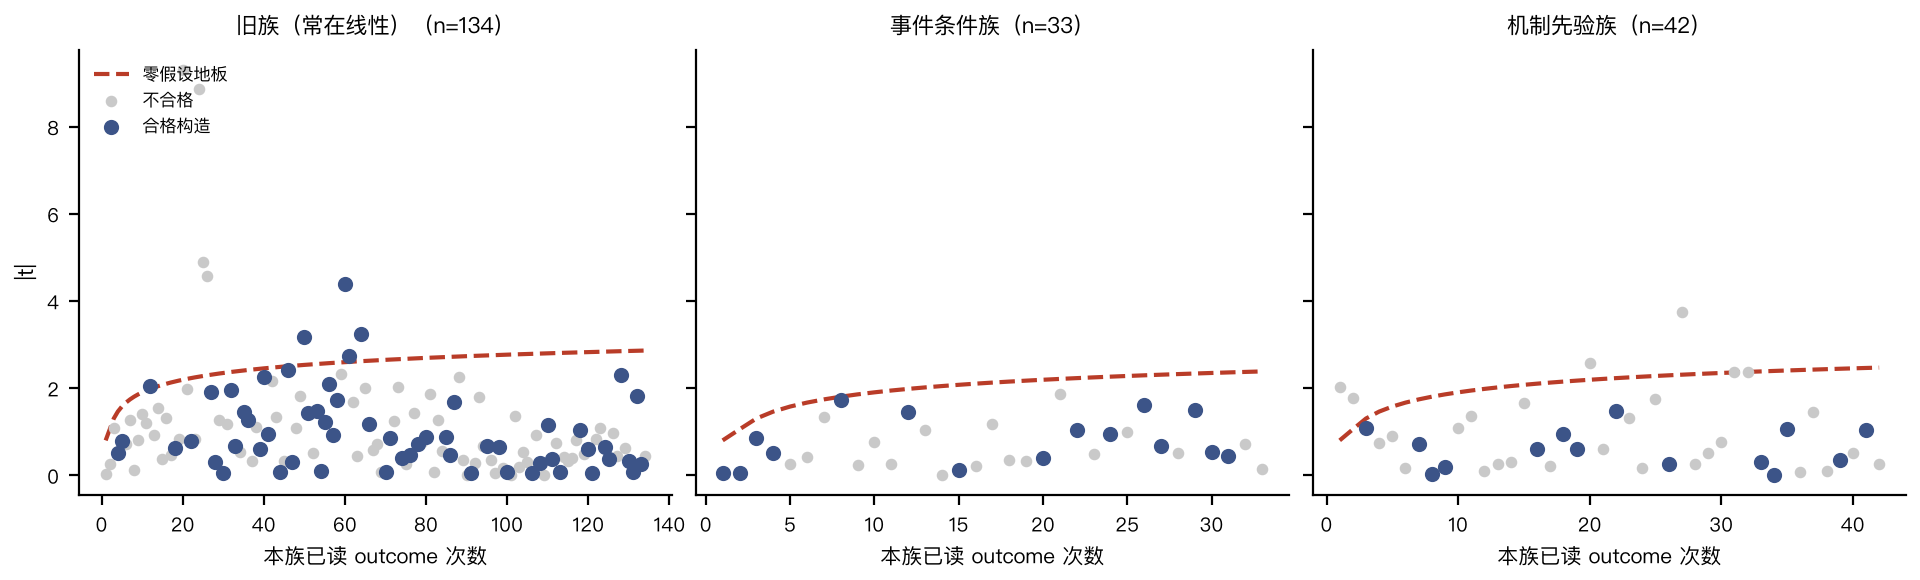
\includegraphics[width=0.95\textwidth]{figures/qualifying_climb.png}
\caption{合格构造的爬升。三栏分别为旧族、事件条件族、机制先验族；虚线为按当时分母算出的
本族地板，深蓝点为合格构造（源含 \texttt{pm\_market} 且符号与预注册方向一致），灰点为不合格者。
栏内分母 134、33、42 为作图时刻只计有 $t$ 统计量的读数。事件条件族与机制先验族的深蓝点
全部在虚线之下；旧族有五个深蓝点在虚线之上，逐条见表~\ref{tab:crossed}。}
\label{fig:climb}
\end{figure}

必须更正一处容易顺口说出的错话：并不是「合格构造从未越线」。旧族有\textbf{五个}合格构造
越过了它们读取时刻的本族地板，分布在三次运行，见表~\ref{tab:crossed}。
成立的说法是加了「并存活」三个字的那一句：五条越线读数没有一条走到最后。
四条在预注册闸门处被拦下，理由与结果高低无关，是样本或推断结构本身不成立；
唯一走完全流程的 \path{run16-study-3} 在一次性的封存段被否决（\S\ref{sec:hero}）。

\begin{table}[htbp]\centering\footnotesize
\begin{tabular}{@{}>{\raggedright\arraybackslash}p{0.18\textwidth} p{0.05\textwidth}
p{0.06\textwidth} p{0.06\textwidth} p{0.06\textwidth}
>{\raggedright\arraybackslash}p{0.45\textwidth}@{}}\toprule
构造 & $n$ & $|t|$ & 地板 & 奖励 & 处置 \\ \midrule
\path{run4-study-4} & 12 & 2.049 & 1.9798 & $+0.07$ &
  置换检验未通过：0.150 的置换斜率不小于实际值；品种维退化 \\
\path{run13-study-1} & 50 & 3.170 & 2.5306 & $+0.64$ &
  观测数 10 低于预注册下限 30，episode 数 7 低于下限 10 \\
\path{run16-study-3} & 60 & 4.393 & 2.5941 & $+1.79$ &
  评价时只因未声明成本模型受阻；成本模型建成后回溯为 candidate（\S\ref{sec:retro}），
  开封后封存段保持率 18.7\%，秩相关同塌，判 sealed\_failed \\
\path{run16-study-4} & 61 & 2.727 & 2.5998 & $+0.13$ & 品种维退化 \\
\path{run16-study-7} & 64 & 3.246 & 2.6163 & $+0.63$ & 品种维退化 \\
\bottomrule\end{tabular}
\caption{越过当时地板的五个合格构造。$n$ 为按 \texttt{outcome\_read} 顺序在本族内的计数，
地板为 $E_2(n)$，奖励为 $|t|$ 减该地板。处置栏文字摘自各条的 \texttt{blocked\_reasons}。
事件条件族与机制先验族至今为零。}
\label{tab:crossed}
\end{table}

把每次运行的合格构造最好奖励按运行顺序排开（此处奖励对照的是读取时刻的\textbf{合并地板}，
即三族分母相加后的那条线，决定 0011 约束 4 要求它随时可读）：
auto $-0.80$、run5 $-1.53$、run11 $-0.09$、run14 $-1.09$、run17 $-1.03$、run23 $-1.11$、
run26 $-0.61$、run28 $-1.84$、run29 $-1.50$、run30 $-1.92$。这串数字在 $-0.1$ 到 $-1.9$
之间横走，没有上行趋势。第二处自我更正在这里：这串数字不是全部。早期有三次运行的
合格最好奖励为正（run4 $+0.07$、run13 $+0.63$、run16 $+1.79$，即表~\ref{tab:crossed} 的三次），
而 run7（$-2.29$）与 run19（$-2.12$）比最近三次运行更低。因此「最近三次最低」的说法不成立，
「在 $-0.1$ 到 $-1.9$ 之间横走」也只对 run22 之后大致成立。

\subsection{门槛在抬，成绩没动}
横走这个词仍然过于宽厚。地板随分母单调上升，维持同样的 $|t|$ 意味着奖励持续下降。
旧族的地板从 2.59（第 60 次读数时）升到 2.8622（第 135 次），机制先验族从 0.7979（第 1 次）
升到 2.4686（第 42 次），而两族的最好合格读数都没有跟着抬。这不是原地踏步，
是门槛在抬而成绩没动。据此，「没有上行趋势」应改写为「与门槛的差距在扩大」。

\subsection{装置确实在变好，但买到的不是信号}
同一批运行里，装置本身的改善有实测数字支持。机械损耗方面，run26 的二十回合中出现三次
provider 修复与一次解析失败，约占四分之一回合；run28 两者都是 0 次，
run30 为解析失败 0 次、provider 修复 2 次（按账本的 \texttt{provider\_repair} 与
\texttt{parse\_failure} 事件计）。搜索广度方面，run26 的全部提案集中在 \path{sc_dominant_t1} 一个品种上，
run28 铺开到 18 个互异品种，run30 为 17 个（按 \texttt{proposal\_locked} 的 \texttt{universe}
字段统计）。机制族使用方面，此前 196 条提案中机制族出现 0 次，run28 的十九条规格全部引用机制族。
方向判据补上之后，run29 的 3 个 candidate 在 run30 归零，同时 run30 出现 14 次
\texttt{direction\_mismatch} 阻断。

这些改善买到的是两样东西：\textbf{测的对象确实是它自称的那个东西}，
以及\textbf{失败能被正确归类}。它们没有买到「更接近找到信号」。
到目前为止最可靠的产出仍然是一批带排除界的否定、四次封存否决，
以及一批被正确识别出来的假象。在「另类数据且符号与自己声明一致」这个最严的口径下，
项目至今没有任何一条构造越过它所在族的地板并存活下来。
